%
\hsection{Installing PostgreSQL under Microsoft Windows}%
%
\begin{figure}%
\centering%
%
\subfloat[][%
We visit the website \url{https://www.postgresql.org/download} and click on~\menu{Windows}.%
\label{fig:installingPostgresWindows01website}%
]{\tightbox{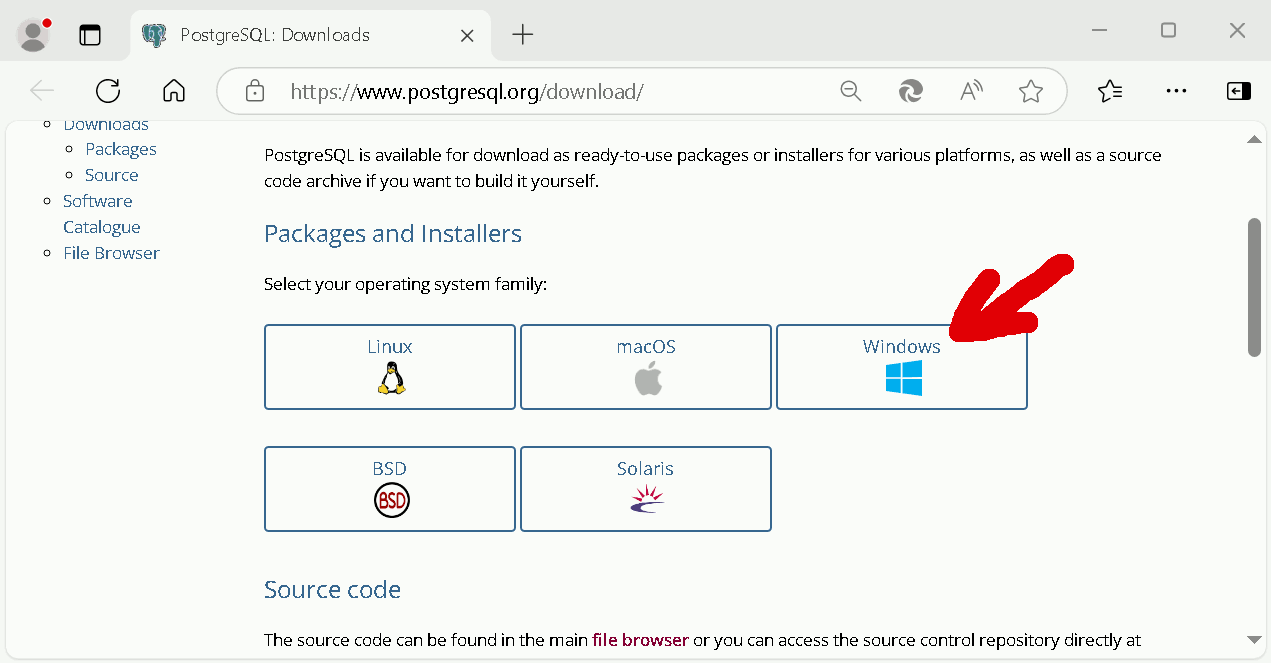
\includegraphics[width=0.7\linewidth]{\currentDir/installingPostgresWindows01website}}}%
%
\floatRowSep
%
\subfloat[][%
We click on the link \emph{download the installer}, which takes us to~\url{https://www.enterprisedb.com/downloads/postgres-postgresql-downloads}.%
\label{fig:installingPostgresWindows02downloadWindows}%
]{\tightbox{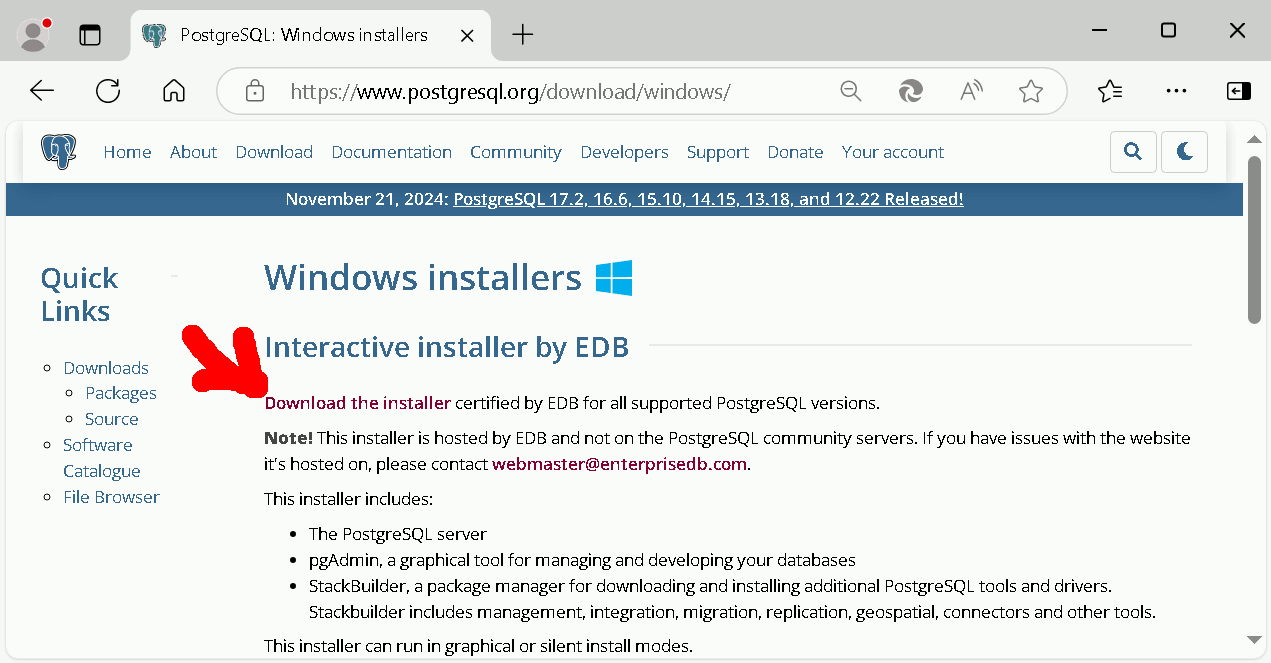
\includegraphics[width=0.7\linewidth]{\currentDir/installingPostgresWindows02downloadWindows}}}%
%
\floatRowSep
%
\subfloat[][%
A wide variety of versions for different \pglspl{OS} are available. %
We choose the newest~(top-most) one for \microsoftWindows, at the time of this writing, this is version~17.2. %
We click the download icon.%
\label{fig:installingPostgresWindows03ebdWebsite}%
]{\tightbox{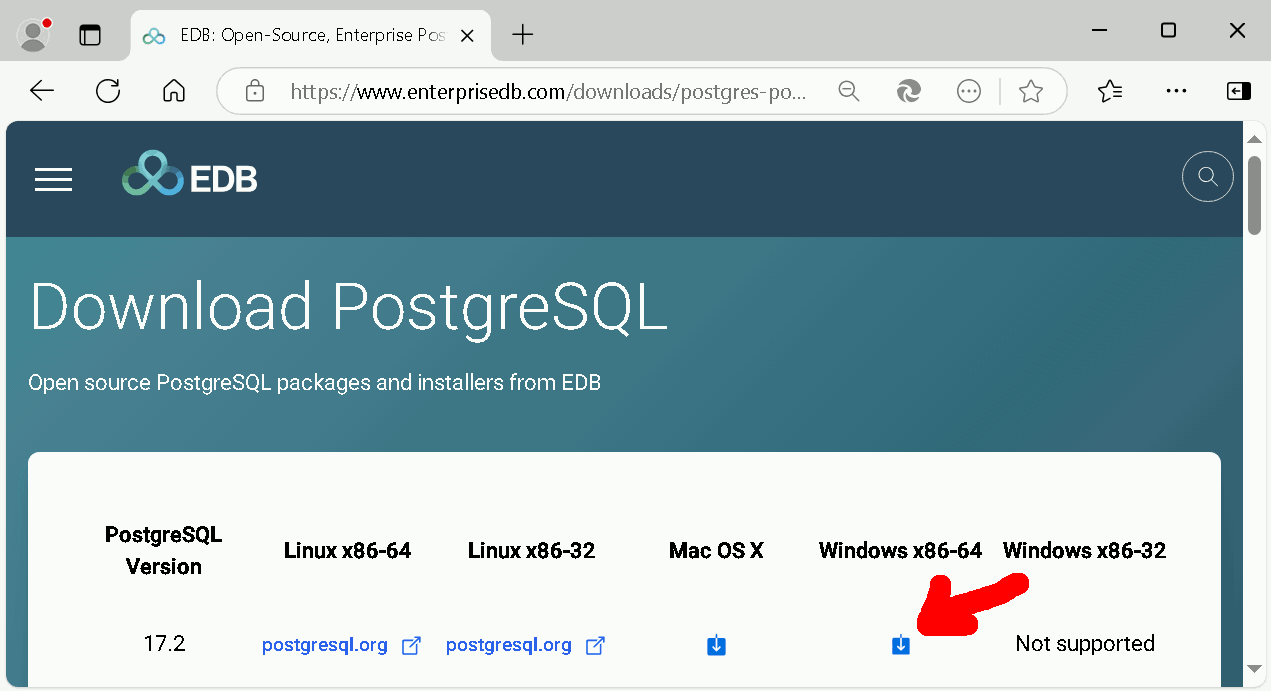
\includegraphics[width=0.7\linewidth]{\currentDir/installingPostgresWindows03ebdWebsite}}}%
%
\caption{Installing and configuring \postgresql\ under \microsoftWindows.}%
\label{fig:installingPostgresWindowsA}%
\end{figure}%
%
\begin{figure}%
\ContinuedFloat%
\centering%
%
\subfloat[][%
The download begins.%
\label{fig:installingPostgresWindows04download}%
]{\tightbox{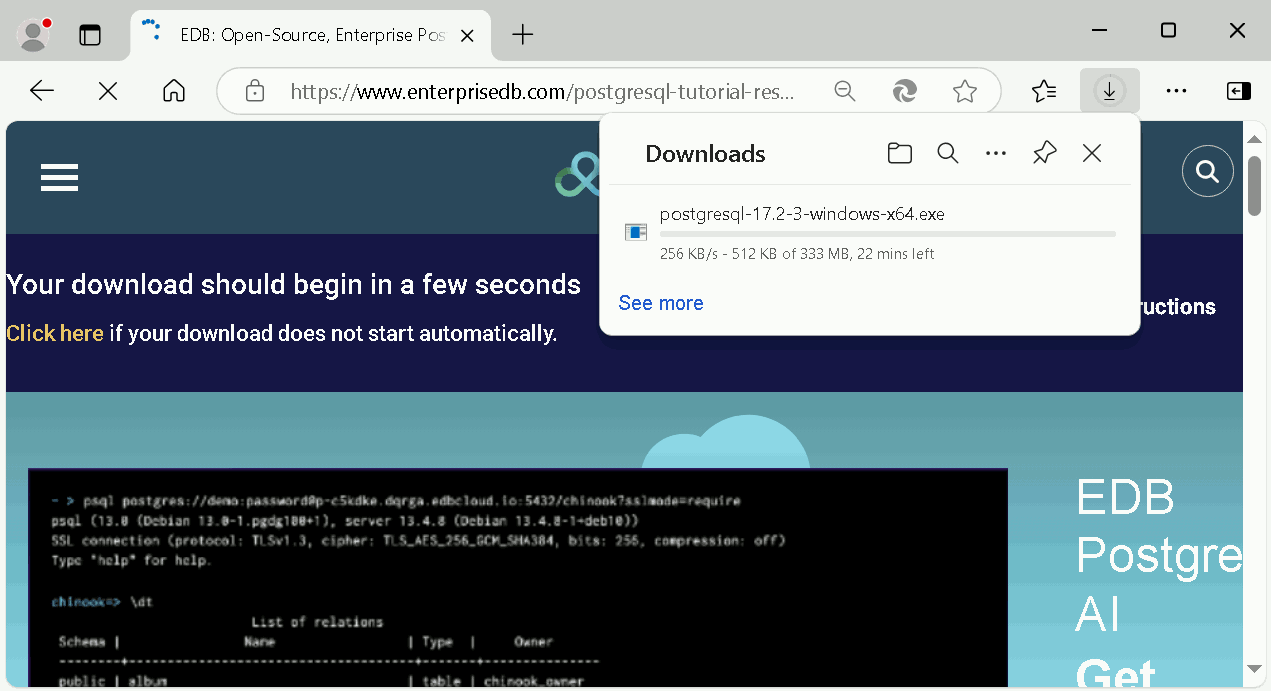
\includegraphics[width=0.7\linewidth]{\currentDir/installingPostgresWindows04download}}}%
%
\floatRowSep%
%
\subfloat[][%
After the download completes, we need to find it\dots%
\label{fig:installingPostgresWindows05downloadsA}%
]{\tightbox{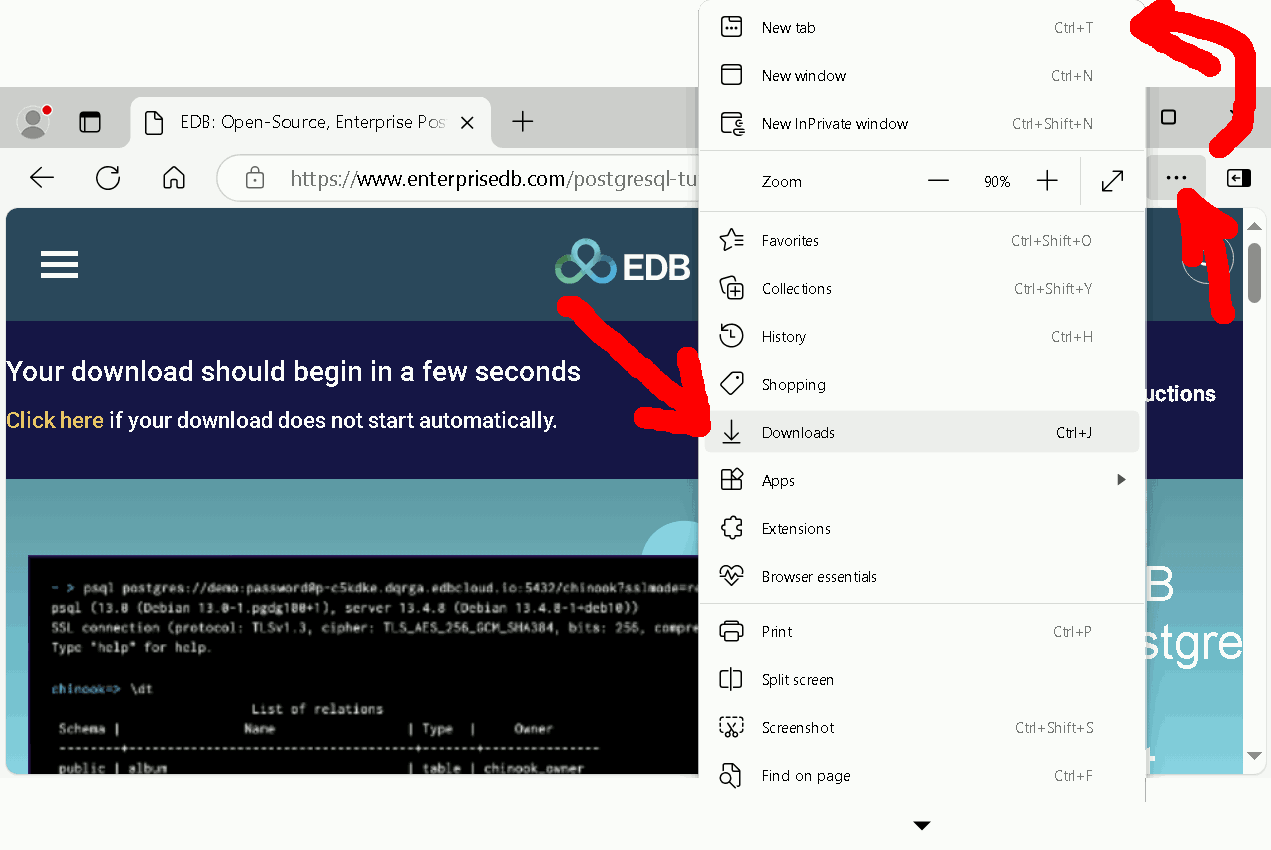
\includegraphics[width=0.7\linewidth]{\currentDir/installingPostgresWindows05downloadsA}}}%
%
\floatRowSep%
%
\subfloat[][%
{\dots}and execute it by clicking on~\menu{Open file}.%
\label{fig:installingPostgresWindows06downloadsB}%
]{\tightbox{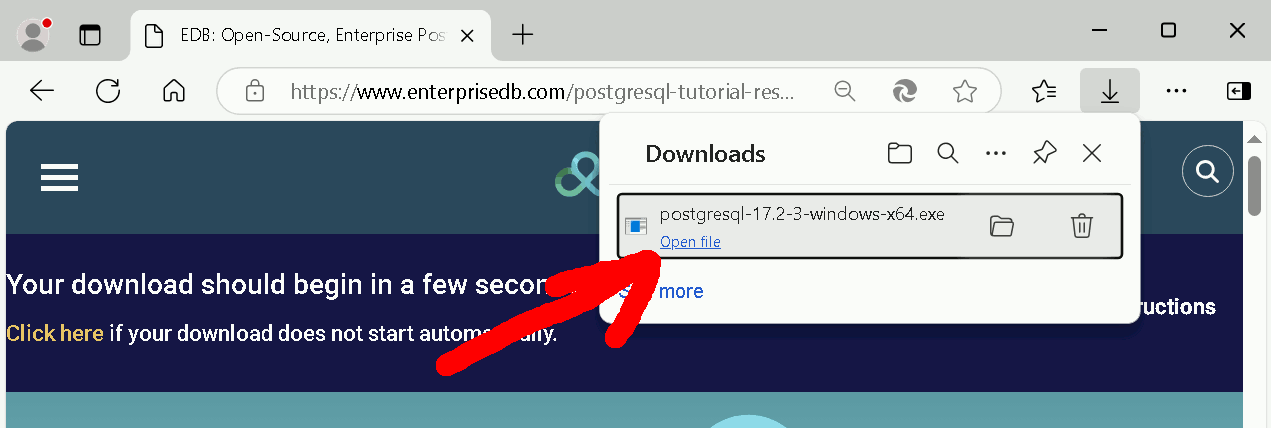
\includegraphics[width=0.7\linewidth]{\currentDir/installingPostgresWindows06downloadsB}}}%
%
\caption{Installing and configuring \postgresql\ under \microsoftWindows~(Continued).}%
\label{fig:installingPostgresWindowsB}%
\end{figure}%
%
\begin{figure}%
\ContinuedFloat%
\centering%
%
\subfloat[][%
When asked whether we want to allow the downloaded program to make changes on our device, we click~\menu{Yes}.%
\label{fig:installingPostgresWindows07install}%
]{\tightbox{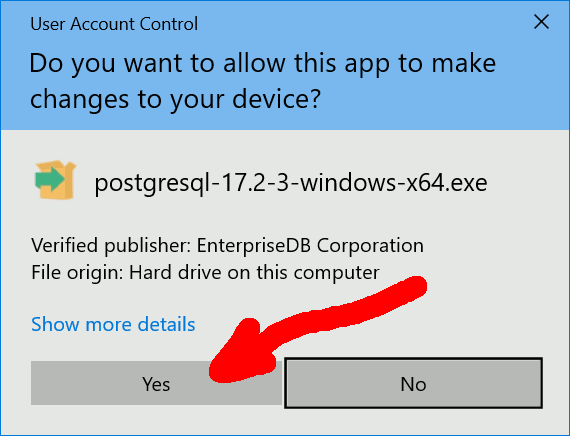
\includegraphics[width=0.475\linewidth]{\currentDir/installingPostgresWindows07install}}}%
%
\floatSep%
%
\subfloat[][%
Then, the installer begins its work.%
\label{fig:installingPostgresWindows08installerStarts}%
]{\tightbox{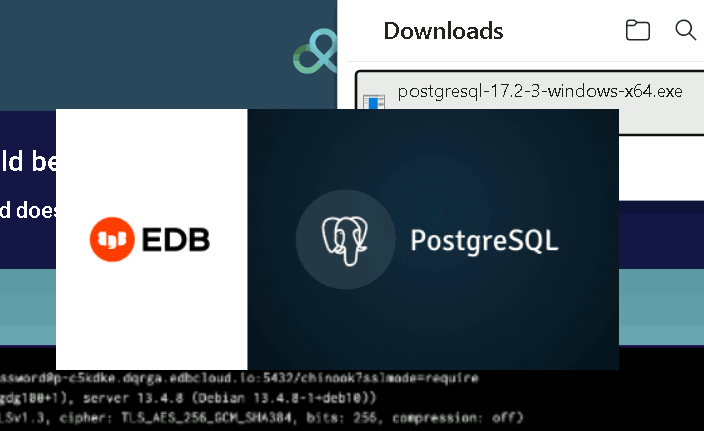
\includegraphics[width=0.475\linewidth]{\currentDir/installingPostgresWindows08installerStarts}}}%
%
\floatRowSep%
%
\subfloat[][%
In the welcome screen, we simply click~\menu{Next}.%
\label{fig:installingPostgresWindows09wizardWelcome}%
]{\tightbox{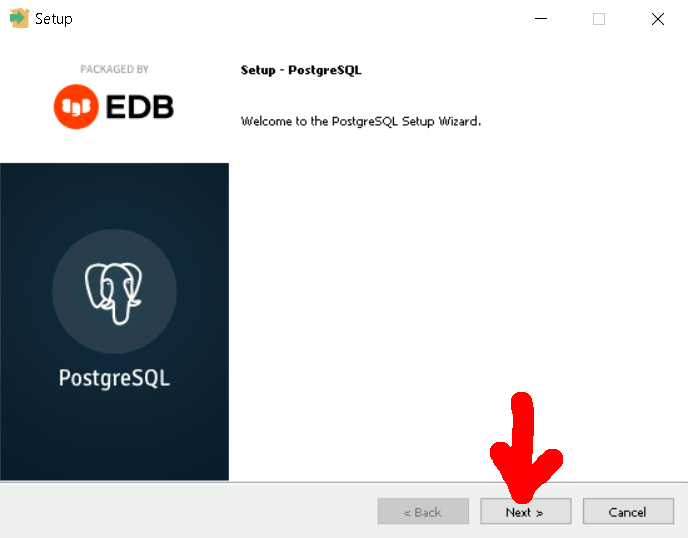
\includegraphics[width=0.475\linewidth]{\currentDir/installingPostgresWindows09wizardWelcome}}}%
%
\floatSep%
%
\subfloat[][%
We can select the directory in which \postgresql\ should be installed. %
Let's leave it at the default setting and click~\menu{Next}.%
\label{fig:installingPostgresWindows10wizardDir}%
]{\tightbox{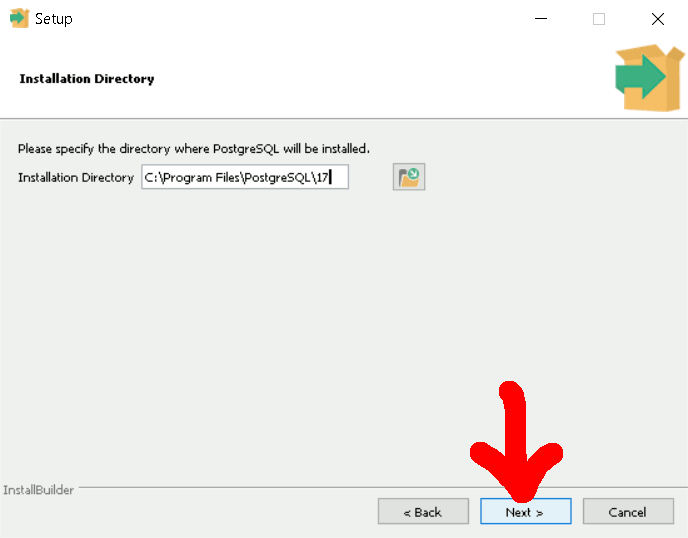
\includegraphics[width=0.475\linewidth]{\currentDir/installingPostgresWindows10wizardDir}}}%
%
\floatRowSep%
%
\subfloat[][%
We now get to the selection of what to install. %
Let's leave it at the default setting and click~\menu{Next}.%
\label{fig:installingPostgresWindows11wizardWhat}%
]{\tightbox{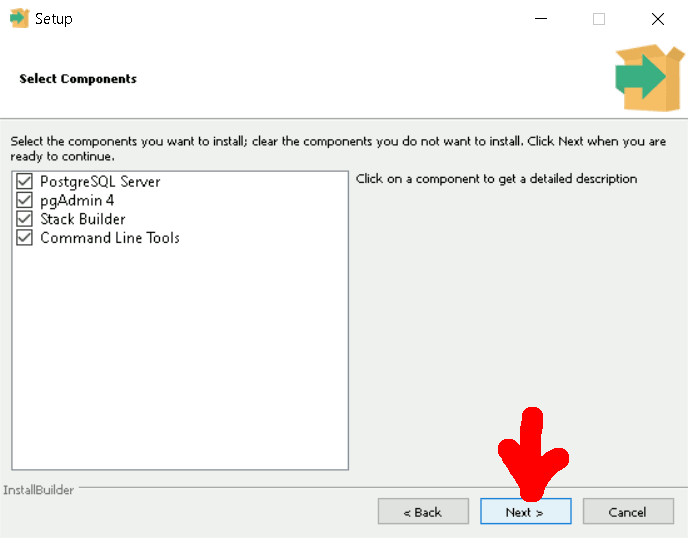
\includegraphics[width=0.475\linewidth]{\currentDir/installingPostgresWindows11wizardWhat}}}%
%
\floatSep%
%
\subfloat[][%
We also leave the directory where the \pglspl{db} will be stored at the default setting and click~\menu{Next}.%
\label{fig:installingPostgresWindows12wizardDataDir}%
]{\tightbox{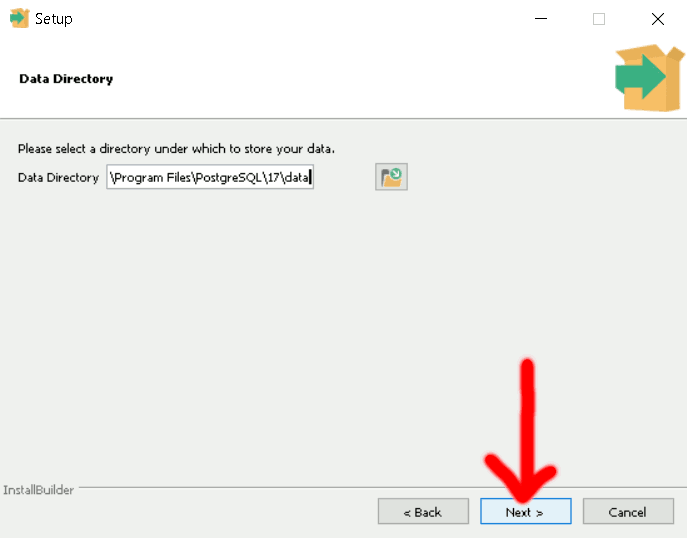
\includegraphics[width=0.475\linewidth]{\currentDir/installingPostgresWindows12wizardDataDir}}}%
%
\caption{Installing and configuring \postgresql\ under \microsoftWindows~(Continued).}%
\label{fig:installingPostgresWindowsC}%
\end{figure}%
%
\begin{figure}%
\ContinuedFloat%
\centering%
%
\subfloat[][%
We need to provide a secure password for the \postgresql\ \pgls{dbms}. %
Please carefully choose one, enter it into both form fields, and click~\menu{Next}.%
\label{fig:installingPostgresWindows13pw}%
]{\tightbox{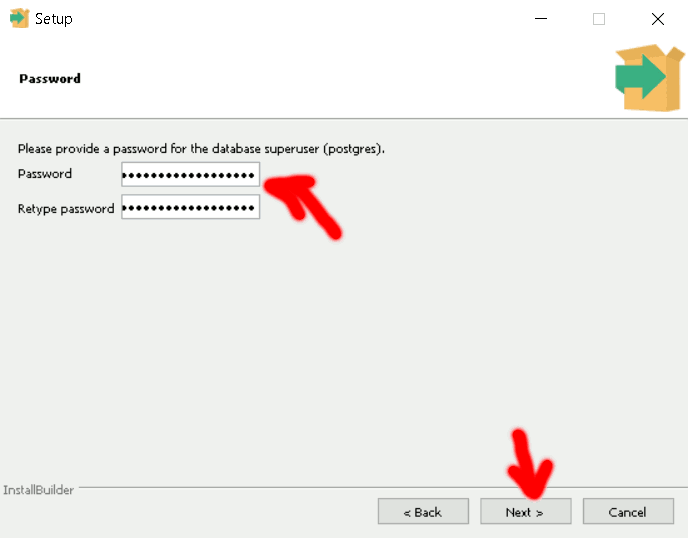
\includegraphics[width=0.475\linewidth]{\currentDir/installingPostgresWindows13pw}}}%
%
\floatSep%
%
\subfloat[][%
We can select the \pgls{port} at which the \postgresql\ \pgls{server} will listen for incoming connections. %
We leave it at the default~5432 and click~\menu{Next}.%
\label{fig:installingPostgresWindows14port}%
]{\tightbox{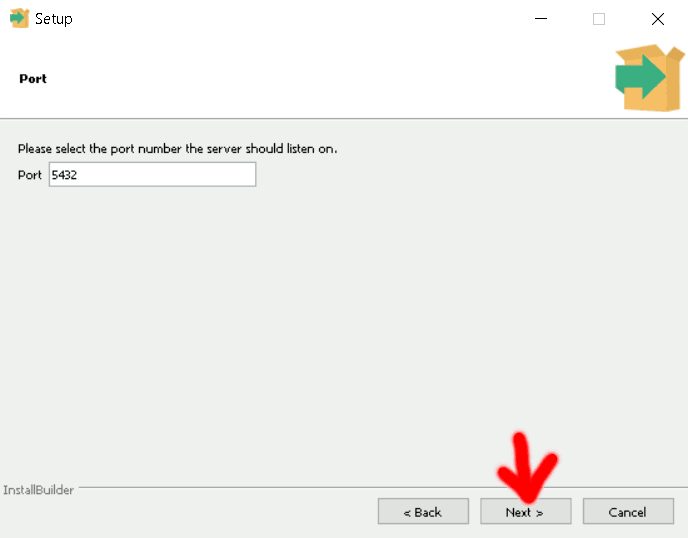
\includegraphics[width=0.475\linewidth]{\currentDir/installingPostgresWindows14port}}}%
%
\floatRowSep%
%
\subfloat[][%
The \pgls{locale} allows us to select country- or culture-specific default settings, e.g., for currency or number formatting. %
We leave it at the system default and click~\menu{Next}.%
\label{fig:installingPostgresWindows15locale}%
]{\tightbox{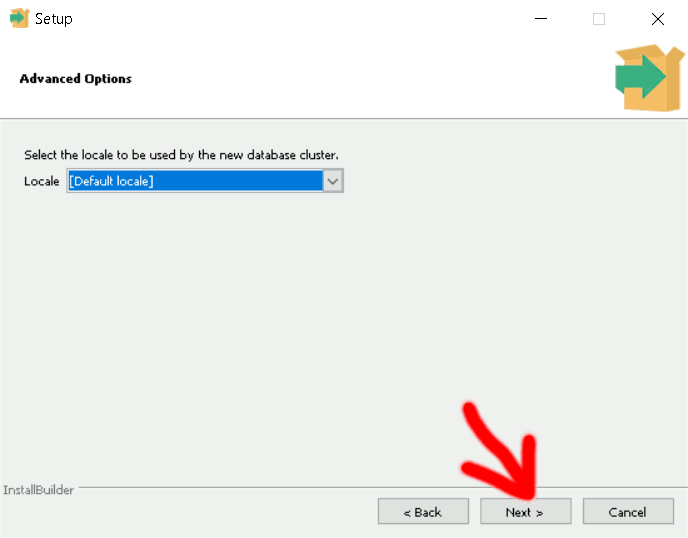
\includegraphics[width=0.475\linewidth]{\currentDir/installingPostgresWindows15locale}}}%
%
\floatSep%
%
\subfloat[][%
We get informed about the components that will be installed. %
We click~\menu{Next}.%
\label{fig:installingPostgresWindows16preInstall}%
]{\tightbox{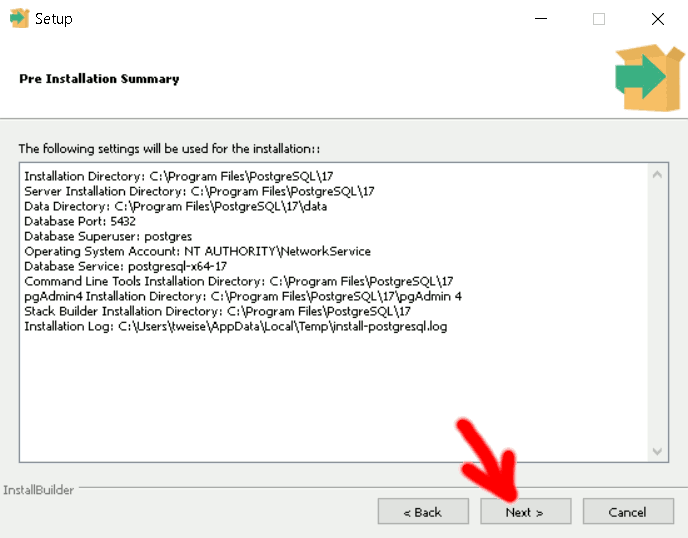
\includegraphics[width=0.475\linewidth]{\currentDir/installingPostgresWindows16preInstall}}}%
%
\floatRowSep%
%
\subfloat[][%
We get asked whether we are ready to install. %
We are, so we click~\menu{Next}.%
\label{fig:installingPostgresWindows17ready}%
]{\tightbox{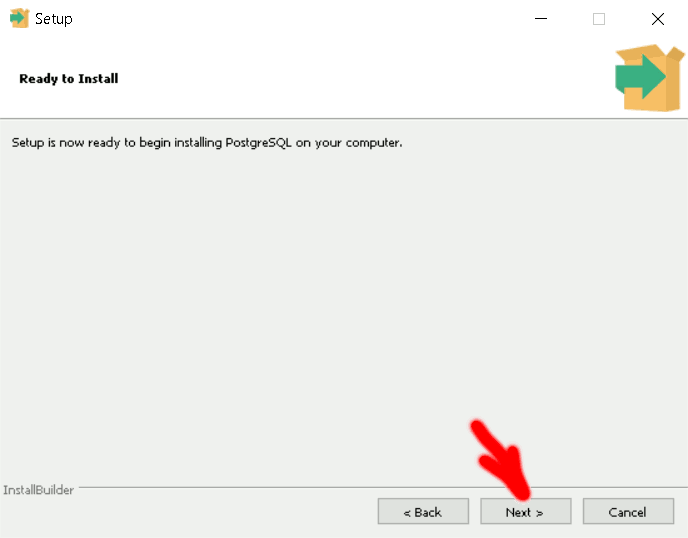
\includegraphics[width=0.475\linewidth]{\currentDir/installingPostgresWindows17ready}}}%
%
\floatSep%
%
\subfloat[][%
The installation begins.%
\label{fig:installingPostgresWindows18installA}%
]{\tightbox{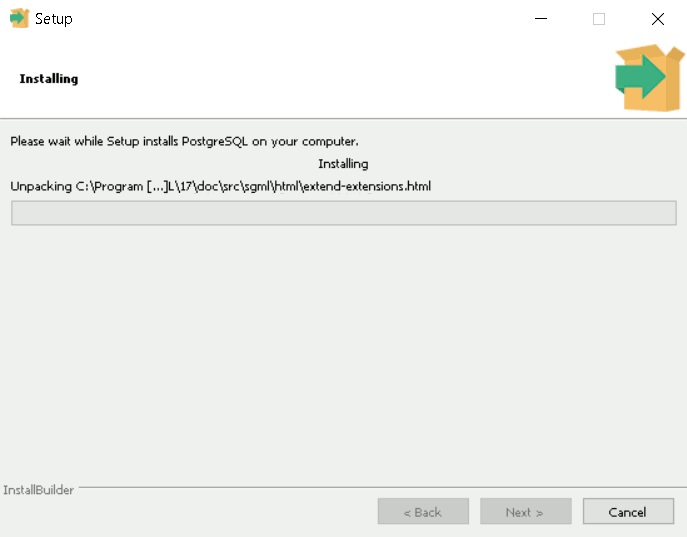
\includegraphics[width=0.475\linewidth]{\currentDir/installingPostgresWindows18installA}}}%
%
\caption{Installing and configuring \postgresql\ under \microsoftWindows~(Continued).}%
\label{fig:installingPostgresWindowsD}%
\end{figure}%
%
\begin{figure}%
\ContinuedFloat%
\centering%
%
\subfloat[][%
The installation proceeds.%
\label{fig:installingPostgresWindows19installB}%
]{\tightbox{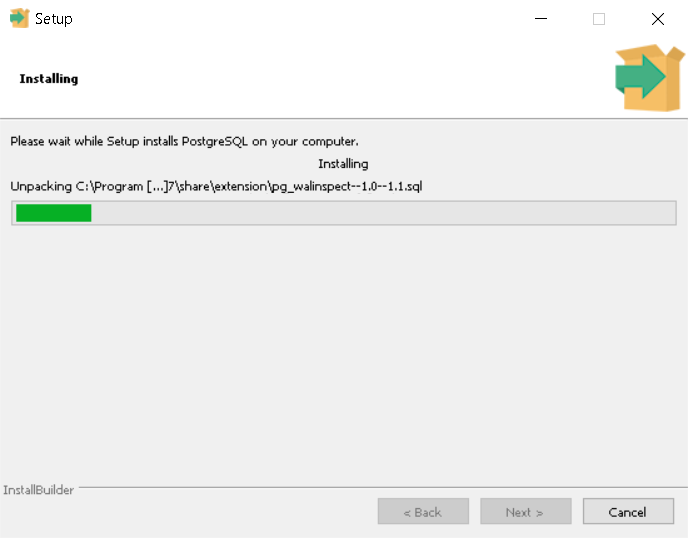
\includegraphics[width=0.475\linewidth]{\currentDir/installingPostgresWindows19installB}}}%
%
\floatSep%
%
\subfloat[][%
Once the installation completes, we get asked whether we want to use the \emph{Stack Builder} software to set up additional components. %
We do not want that, so we make sure that the checkbox is \emph{not} checked. %
Then we click~\menu{Finish}. %
\postgresql\ is now installed.%
\label{fig:installingPostgresWindows20finish}%
]{\tightbox{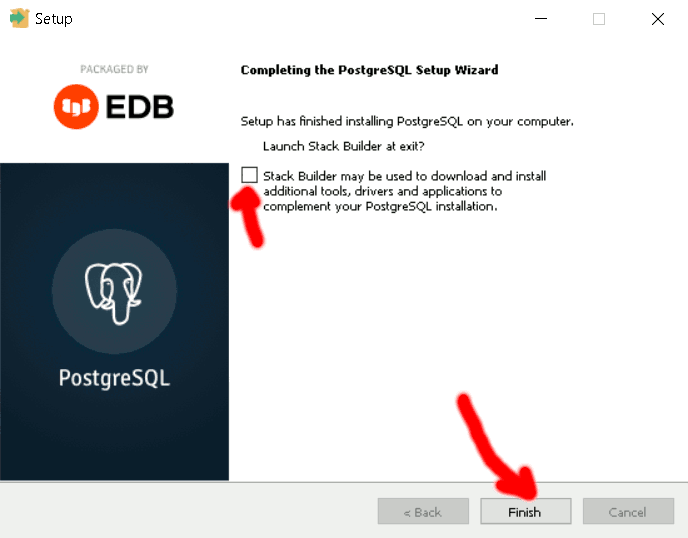
\includegraphics[width=0.475\linewidth]{\currentDir/installingPostgresWindows20finish}}}%
%
\floatRowSep%
%
\subfloat[][%
To validate the installation, we need to open a \pgls{terminal}. %
We therefore press \keys{\OSwin + R}.%
\label{fig:installingPostgresWindows21windowsR}%
]{\tightbox{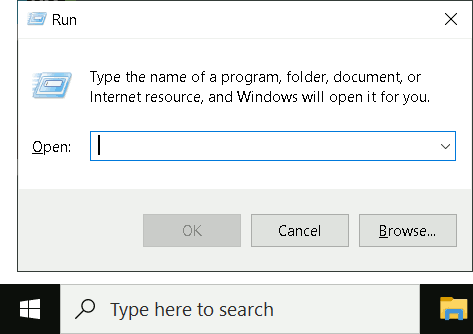
\includegraphics[width=0.475\linewidth]{\currentDir/installingPostgresWindows21windowsR}}}%
%
\floatSep%
%
\subfloat[][%
We type in \textil{cmd} and hit~\keys{\return}.%
\label{fig:installingPostgresWindows22cmd}%
]{\tightbox{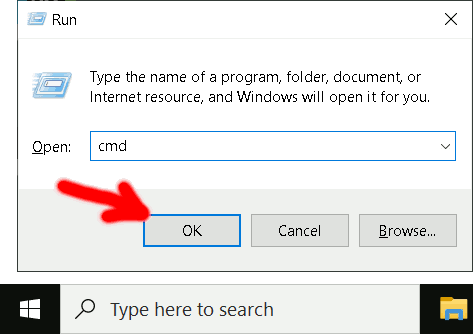
\includegraphics[width=0.475\linewidth]{\currentDir/installingPostgresWindows22cmd}}}%
%
\floatRowSep%
%
\subfloat[][%
A new \pgls{terminal} window opens up.%
\label{fig:installingPostgresWindows23terminal}%
]{\tightbox{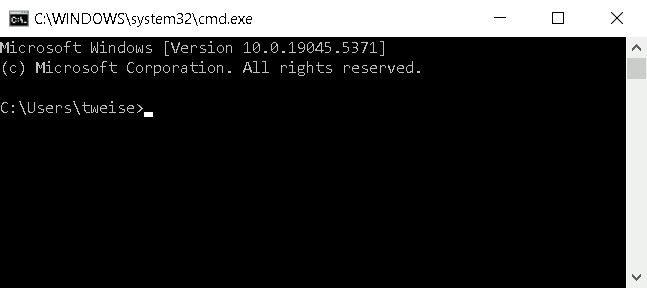
\includegraphics[width=0.7\linewidth]{\currentDir/installingPostgresWindows23terminal}}}%
%
%
\caption{Installing and configuring \postgresql\ under \microsoftWindows~(Continued).}%
\label{fig:installingPostgresWindowsE}%
\end{figure}%
%
\begin{figure}%
\ContinuedFloat%
\centering%
%
\subfloat[][%
We need to enter the \batil{bin}~folder in the directory into where the \postgresql\ \pgls{dbms} was installed. %
If we used the default settings, we can do that by typing~\batil{cd "C:\\Program Files\\PostgreSQL\\bin"} and hitting~\keys{\return}.%
\label{fig:installingPostgresWindows24cd}%
]{\tightbox{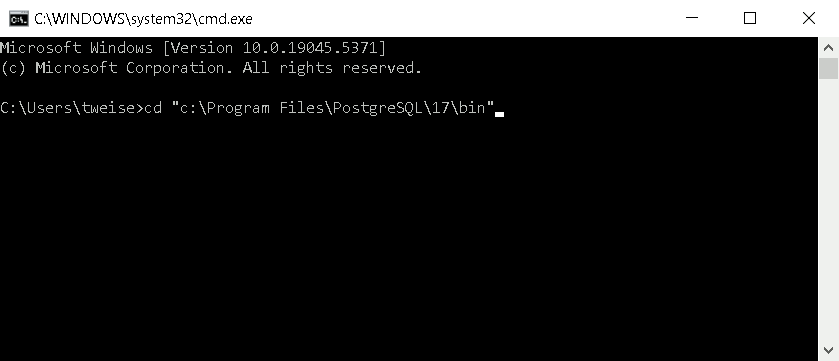
\includegraphics[width=0.7\linewidth]{\currentDir/installingPostgresWindows24cd}}}%
%
\floatRowSep%
%
\subfloat[][%
We are now in that directory.%
\label{fig:installingPostgresWindows25inDir}%
]{\tightbox{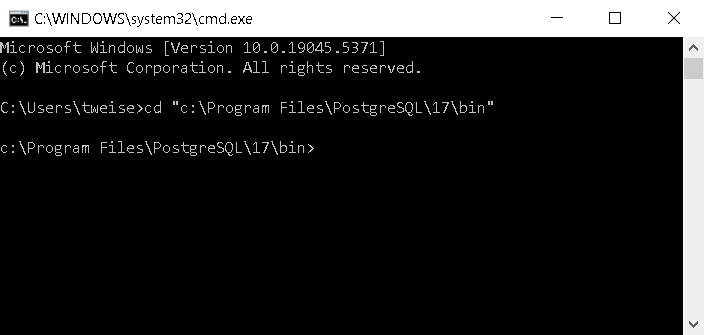
\includegraphics[width=0.7\linewidth]{\currentDir/installingPostgresWindows25inDir}}}%
%
\floatRowSep%
%
\subfloat[][%
First, we want to print the version of \psql, the \pgls{client} program of \postgresql. %
We can do this by typing \batil{psql -V} and pressing~\keys{\return}.%
\label{fig:installingPostgresWindows26psqlV}%
]{\tightbox{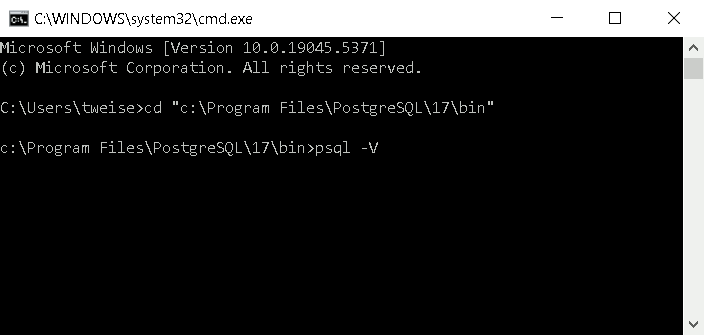
\includegraphics[width=0.7\linewidth]{\currentDir/installingPostgresWindows26psqlV}}}%
%
%
\caption{Installing and configuring \postgresql\ under \microsoftWindows~(Continued).}%
\label{fig:installingPostgresWindowsF}%
\end{figure}%
%
\begin{figure}%
\ContinuedFloat%
\centering%
%
\subfloat[][%
In my case, the output shows that version~17.2 was installed.%
\label{fig:installingPostgresWindows27psqlVres}%
]{\tightbox{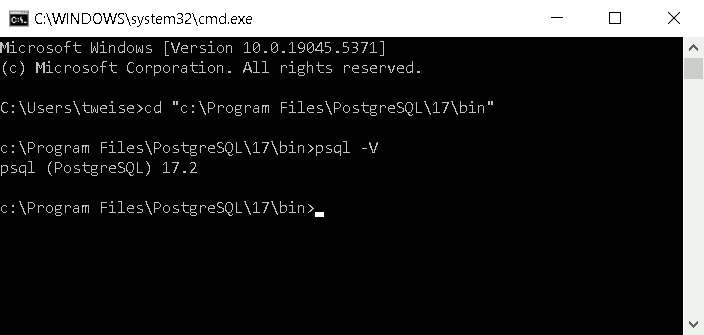
\includegraphics[width=0.7\linewidth]{\currentDir/installingPostgresWindows27psqlVres}}}%
%
\floatRowSep%
%
\subfloat[][%
We now want to also see which version of the \postgresql\ \pgls{server} was installed and, by doing so, also confirm that the server is up and running correctly. %
We therefore launch \batil{psql -U postgres}, i.e., start \psql\ using the user~(or role) \textil{postgres}.%
\label{fig:installingPostgresWindows28psqlU}%
]{\tightbox{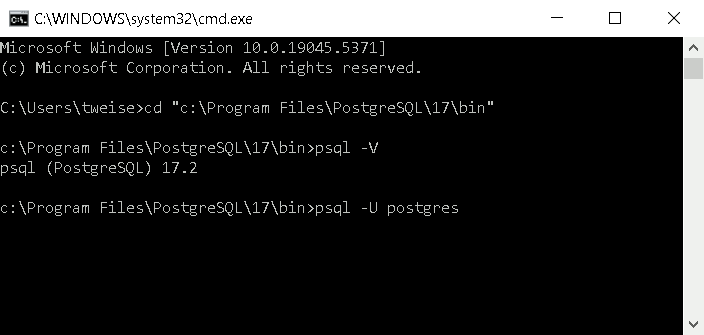
\includegraphics[width=0.7\linewidth]{\currentDir/installingPostgresWindows28psqlU}}}%
%
\floatRowSep%
%
\subfloat[][%
When the program starts, it requires us to enter the password for the user \textil{postgres}. %
This is the password that we specified during the installation in \cref{fig:installingPostgresWindows13pw}. %
We enter it and press~\keys{\return}. %
We are now in the \psql\ console, and see the \textil{postgres=\#} prompt.%
\label{fig:installingPostgresWindows29pw}%
]{\tightbox{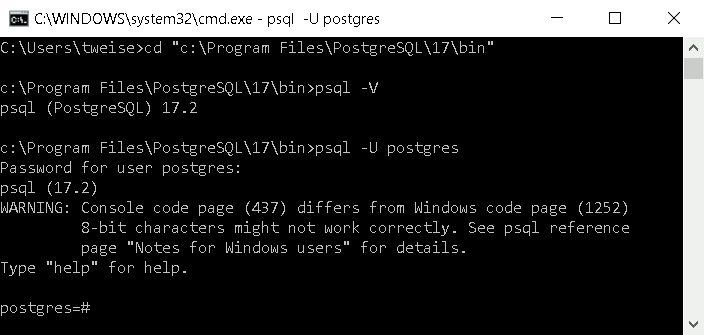
\includegraphics[width=0.7\linewidth]{\currentDir/installingPostgresWindows29pw}}}%
%
%
\caption{Installing and configuring \postgresql\ under \microsoftWindows~(Continued).}%
\label{fig:installingPostgresWindowsG}%
\end{figure}%
%
\begin{figure}%
\ContinuedFloat%
\centering%
%
\subfloat[][%
We enter the \sql\ command \sqlil{SELECT * FROM VERSION();} and press~\keys{\return}.%
\label{fig:installingPostgresWindows30selectVer}%
]{\tightbox{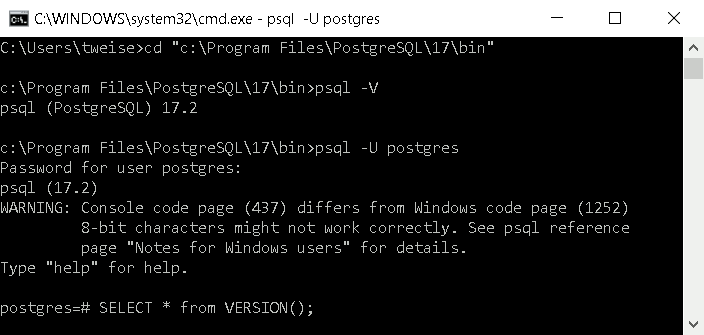
\includegraphics[width=0.7\linewidth]{\currentDir/installingPostgresWindows30selectVer}}}%
%
\floatRowSep%
%
\subfloat[][%
The result gets printed. %
In my case, it shows that the \postgresql\ \pgls{server} also has version~17.2.%
We now type in~\keys{\textbackslash+q+\return}, which will exits~\psql.%
\label{fig:installingPostgresWindows31verResQ}%
]{\tightbox{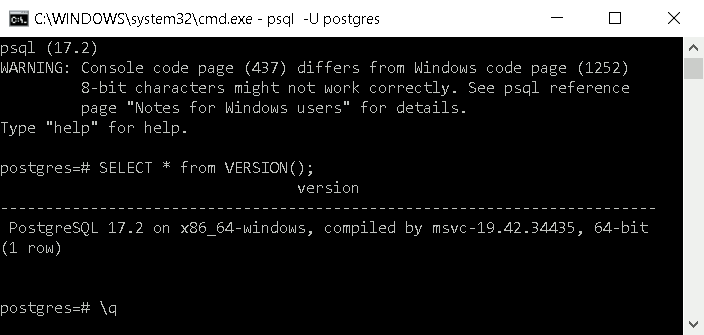
\includegraphics[width=0.7\linewidth]{\currentDir/installingPostgresWindows31verResQ}}}%
%
\floatRowSep%
%
\subfloat[][%
Let us now explore how the \postgresql\ \pgls{server} is run on our \microsoftWindows\ machine: %
It is executed as a service. %
We press~\keys{\OSwin}, type in \textil{services}, and click on the \inQuotes{gears} symbol named \emph{Services} that appears.%
\label{fig:installingPostgresWindows32services}%
]{\tightbox{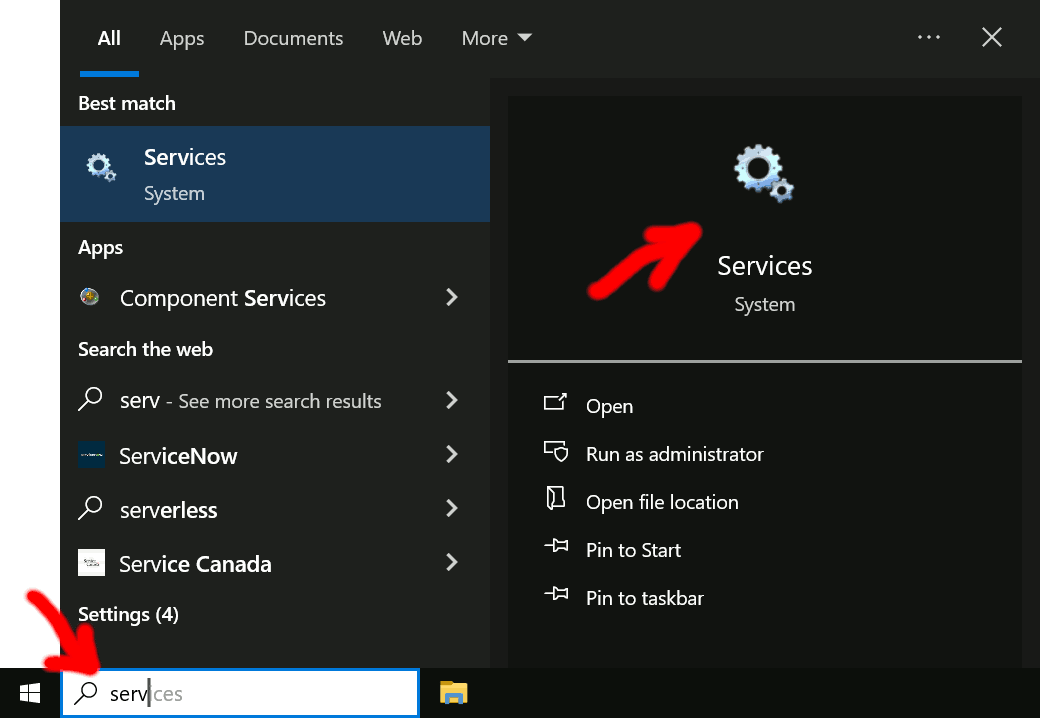
\includegraphics[width=0.7\linewidth]{\currentDir/installingPostgresWindows32services}}}%
%
\caption{Installing and configuring \postgresql\ under \microsoftWindows~(Continued).}%
\label{fig:installingPostgresWindowsH}%
\end{figure}%
%
\begin{figure}%
\ContinuedFloat%
\centering%
%
\subfloat[][%
The \emph{Services} system setup window opens. %
Search for a service named something like \postgresql, in my case, it is~\textil{postgresql-x64-17}. %
Right-click on it.%%
\label{fig:installingPostgresWindows33servicesPostgres}%
]{\tightbox{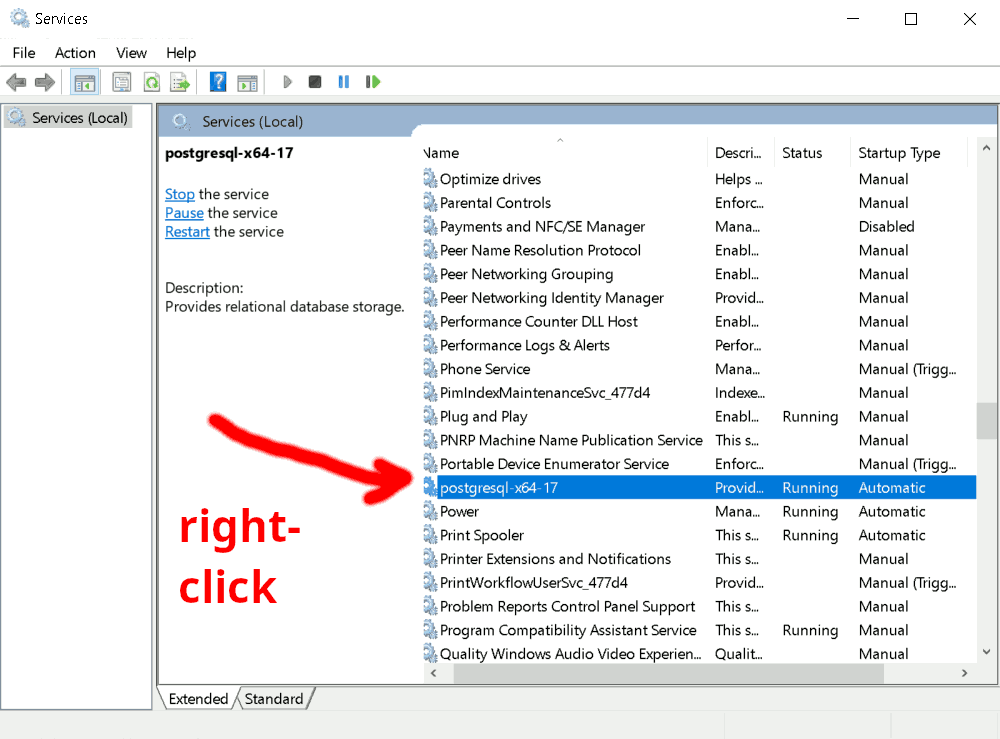
\includegraphics[width=0.8\linewidth]{\currentDir/installingPostgresWindows33servicesPostgres}}}%
%
\floatRowSep%
%
\subfloat[][%
In the Pop-up menu that appears, click on~\menu{Properties}.%
\label{fig:installingPostgresWindows34servicesProperties}%
]{\tightbox{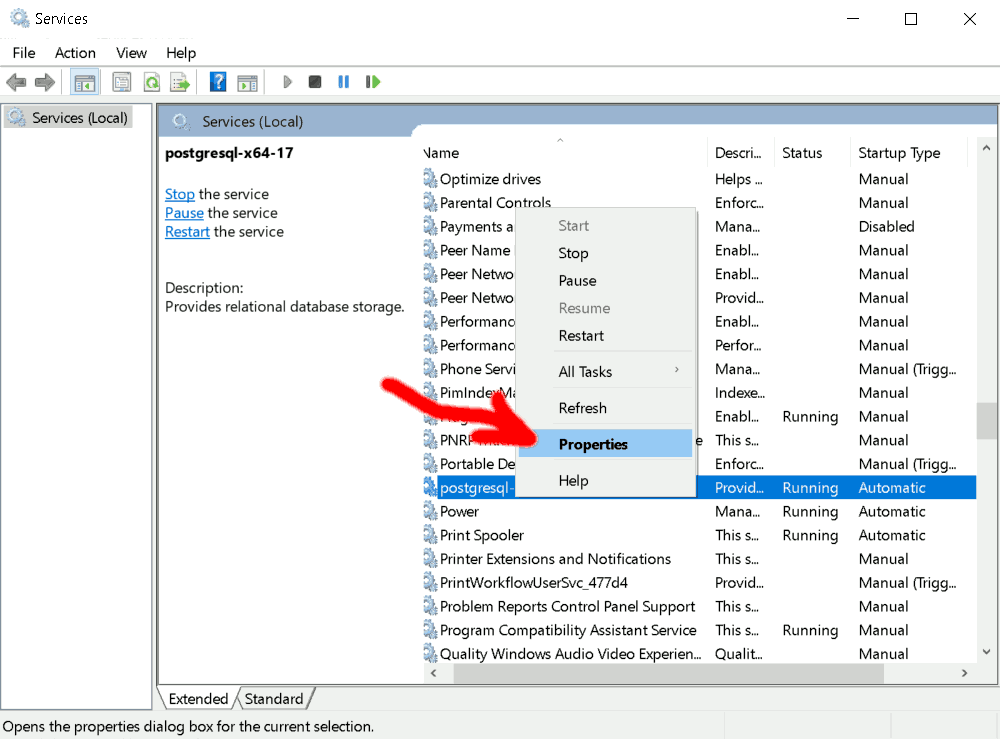
\includegraphics[width=0.8\linewidth]{\currentDir/installingPostgresWindows34servicesProperties}}}%
%
\caption{Installing and configuring \postgresql\ under \microsoftWindows~(Continued).}%
\label{fig:installingPostgresWindowsI}%
\end{figure}%
%
\begin{figure}%
\ContinuedFloat%
\centering%
%
\subfloat[][%
The service properties dialog appears.%
\label{fig:installingPostgresWindows35servicesPropertiesPostgres}%
]{\tightbox{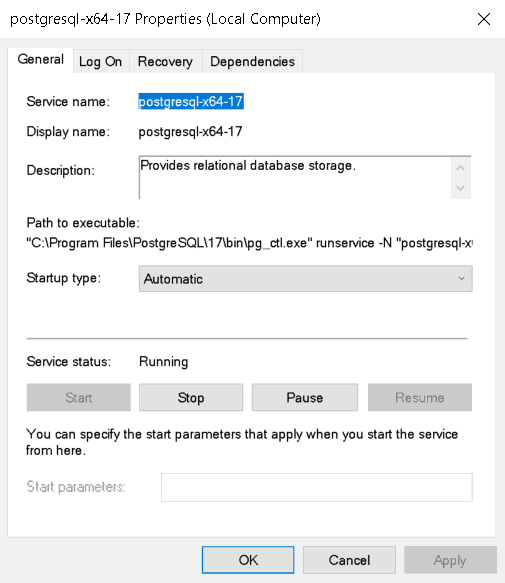
\includegraphics[width=0.475\linewidth]{\currentDir/installingPostgresWindows35servicesPropertiesPostgres}}}%
%
\floatSep%
%
\subfloat[][%
Click on the drop-down box for~\menu{Startup type:}. %
It will be set to~\menu{Automatic}, which means that the \postgresql\ \pgls{dbms} \pgls{server} will be started automatically whenever your system starts.%
\label{fig:installingPostgresWindows36servicesStartupType}%
]{\tightbox{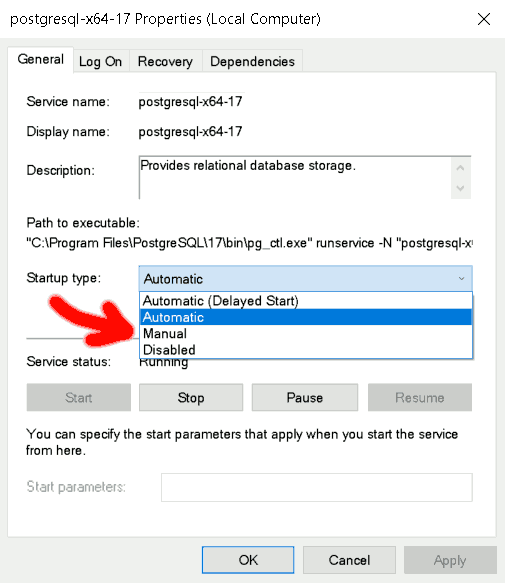
\includegraphics[width=0.475\linewidth]{\currentDir/installingPostgresWindows36servicesStartupType}}}%
%
\floatRowSep%
%
\subfloat[][%
The following is completely optional.
You do not have to do that.
If you do \emph{not} want that, because it may make booting slower and maybe you only need the service studying for this course, you can turn off this automated startup. %
You would therefore select~\menu{Manual} as~\menu{Startup type:} and click the \menu{Apply}~button.%
\label{fig:installingPostgresWindows37servicesManual}%
]{\tightbox{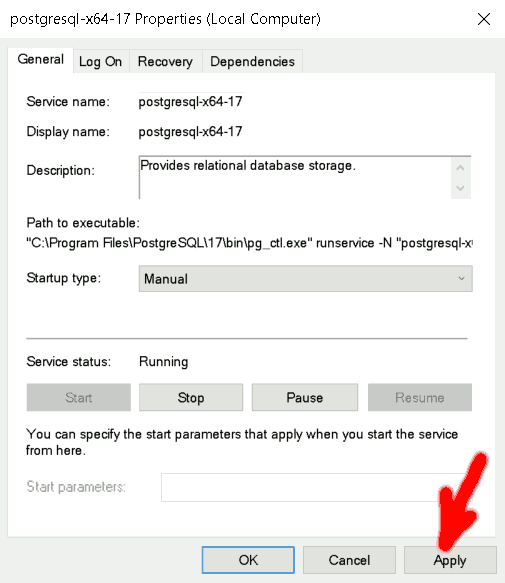
\includegraphics[width=0.475\linewidth]{\currentDir/installingPostgresWindows37servicesManual}}}%
%
\floatSep%
%
\subfloat[][%
The service is currently still running after that change, but it will not start automatically anymore. %
If you want it to start automatically again, just select~\menu{Automatic} as~\menu{Startup type:}. %
If you want to stop the currently-running service, click the \menu{Stop}~button.%
\label{fig:installingPostgresWindows38servicesStop}%
]{\tightbox{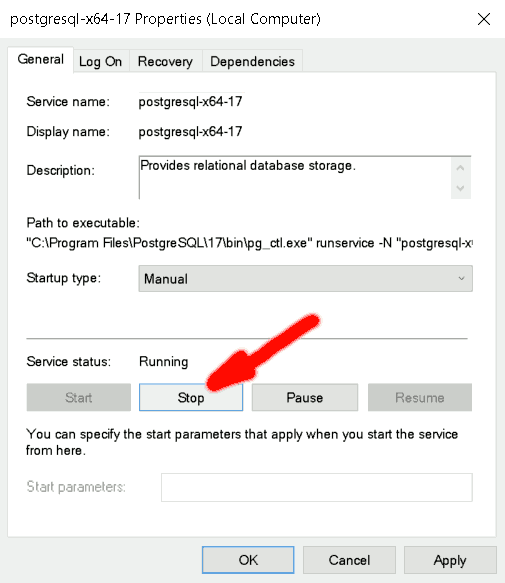
\includegraphics[width=0.475\linewidth]{\currentDir/installingPostgresWindows38servicesStop}}}%
%
\caption{Installing and configuring \postgresql\ under \microsoftWindows~(Continued).}%
\label{fig:installingPostgresWindowsJ}%
\end{figure}%
%
\begin{figure}%
\ContinuedFloat%
\centering%
%
\subfloat[][%
Then, the service will be stopped.%
\label{fig:installingPostgresWindows39servicesStopping}%
]{\tightbox{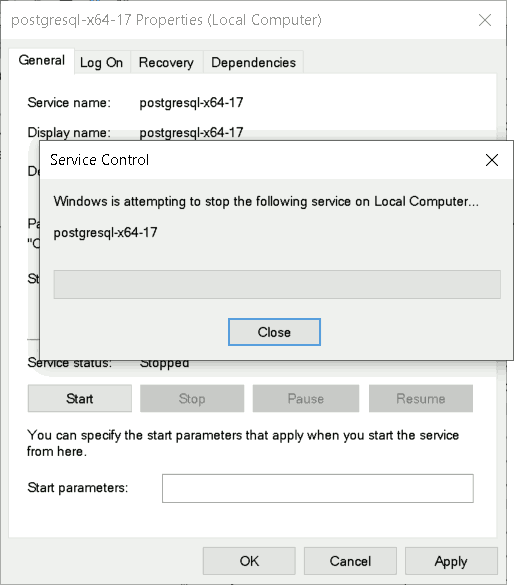
\includegraphics[width=0.475\linewidth]{\currentDir/installingPostgresWindows39servicesStopping}}}%
%
\floatSep%
%
\subfloat[][%
It is now no longer running. %
Let's start it again by clicking the \menu{Start}~button.%
\label{fig:installingPostgresWindows40servicesStart}%
]{\tightbox{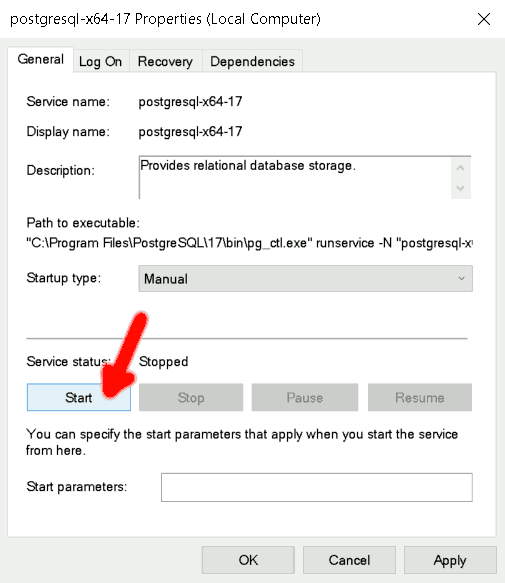
\includegraphics[width=0.475\linewidth]{\currentDir/installingPostgresWindows40servicesStart}}}%
%
\floatRowSep%
%
\subfloat[][%
The service is now starting again.%
\label{fig:installingPostgresWindows41servicesStarting}%
]{\tightbox{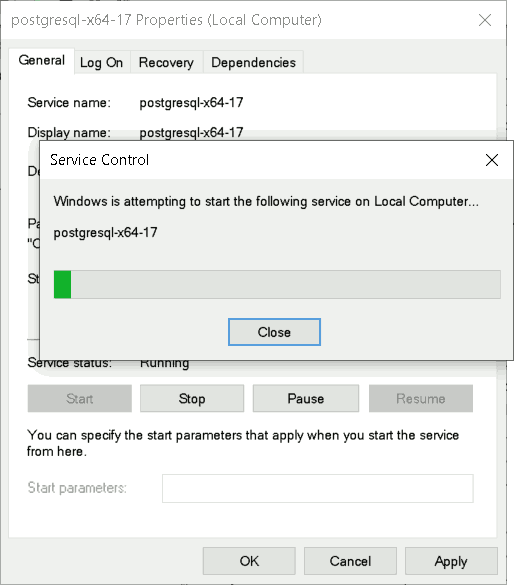
\includegraphics[width=0.475\linewidth]{\currentDir/installingPostgresWindows41servicesStarting}}}%
%
\floatSep%
%
\subfloat[][%
We click \menu{OK} to leave the dialog.%
\label{fig:installingPostgresWindows42servicesOK}%
]{\tightbox{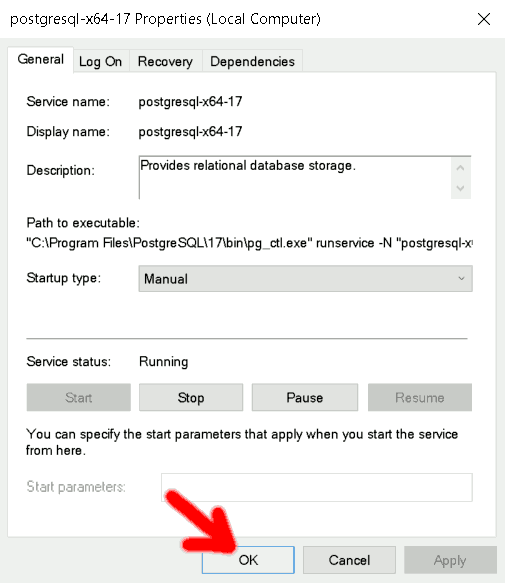
\includegraphics[width=0.475\linewidth]{\currentDir/installingPostgresWindows42servicesOK}}}%
%
\caption{Installing and configuring \postgresql\ under \microsoftWindows~(Continued).}%
\label{fig:installingPostgresWindowsK}%
\end{figure}%
%
\begin{figure}%
\ContinuedFloat%
\centering%
%
\subfloat[][%
We see that the service is \emph{Running} and in mode \emph{Manual}~(if we changed it to that mode). %
When you shutdown your system, the \pgls{dbms} is stopped. %
It does not start automatically when you boot~(unless you set \emph{Automatic} as \emph{Startup type}). %
So if you need it, you would again enter the \emph{Services} system setup program and manually start it.%
\label{fig:installingPostgresWindows43services}%
]{\tightbox{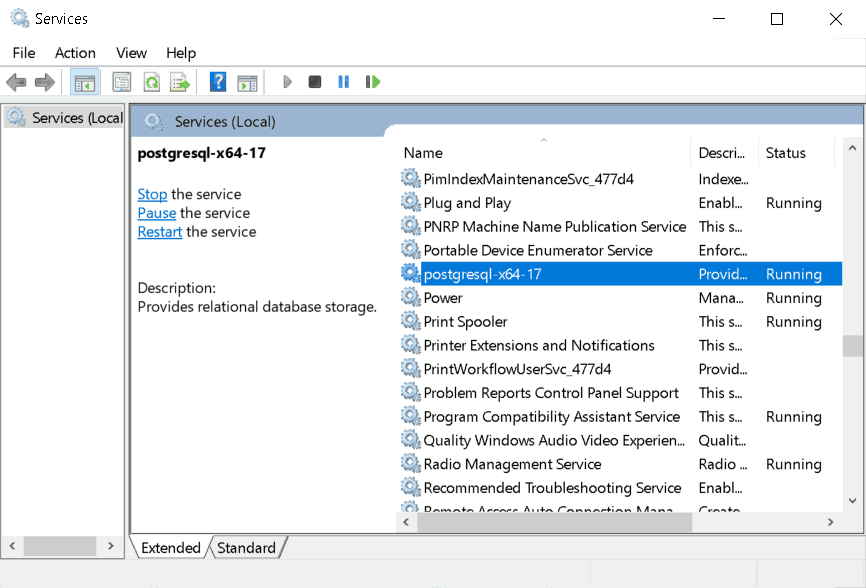
\includegraphics[width=0.8\linewidth]{\currentDir/installingPostgresWindows43services}}}%
%
\caption{Installing and configuring \postgresql\ under \microsoftWindows~(Continued).}%
\label{fig:installingPostgresWindowsL}%
\end{figure}%
%
%
We want to install and properly configure \postgresql\ on a \microsoftWindows\ system.
To do this, we first visit the official download page at~\url{https://www.postgresql.org/download}, as shown in \cref{fig:installingPostgresWindows01website}.
There, we click on the large \emph{Windows}~\keys{\OSwin} menu.
This leads to a page with more text and the link \emph{download the installer}~(\cref{fig:installingPostgresWindows02downloadWindows}).
This, in turn, takes us to~\url{https://www.enterprisedb.com/downloads/postgres-postgresql-downloads}, as shown in \cref{fig:installingPostgresWindows03ebdWebsite}.

On this website, a wide variety of different versions of \postgresql\ for different \pglspl{OS} can be downloaded.
We choose the newest version for \microsoftWindows, which can be found in the top-most row of the list presented to us.
At the time of this writing, this is version~17.2.
We click the corresponding download icon.

The download begins, as shown in~\cref{fig:installingPostgresWindows04download}.
Once it completes, we need to find the downloaded file, as shown in \cref{fig:installingPostgresWindows05downloadsA}.
I downloaded the software using the Microsoft Edge browser, so I need to click on the \keys{\dots}~button and then on \menu{Downloads}, or press~\keys{\ctrl+J}.
Regardless how you downloaded the installer file, once you found it, you need to execute it.
As shown in \cref{fig:installingPostgresWindows06downloadsB}, this can be accomplished by clicking on~\menu{Open file} in my case.
The \pgls{OS} will now ask us whether we want to permit the downloaded program to make changes on our device.
We certainly want that, because we want to use it to install \postgresql.
So we click~\menu{Yes} in \cref{fig:installingPostgresWindows07install}.

Then, the installer begins its work with a small splash screen shown in \cref{fig:installingPostgresWindows08installerStarts}.
In the following welcome screen, we simply click~\menu{Next}~(\cref{fig:installingPostgresWindows09wizardWelcome}).
We now work our way through setting up the installation options step-by-step.
First, we can select the directory in which \postgresql\ should be installed in \cref{fig:installingPostgresWindows10wizardDir}.
I chose to just leave it at the default setting and click~\menu{Next}.
This is what I will do for most of the rest of the installation, too.

We now get to the selection of what to install.
I left this at the default setting, too, and simply click~\menu{Next} in \cref{fig:installingPostgresWindows11wizardWhat}.
Then, in \cref{fig:installingPostgresWindows12wizardDataDir}, we can also leave the directory where the \pglspl{db} will be stored at the default setting and click~\menu{Next}.

In the following screen, we do need to provide a secure password for the \postgresql\ \pgls{dbms}.
Here we need to carefully choose a password \emph{and remember it well}.
We enter it into both form fields, and click~\menu{Next} in \cref{fig:installingPostgresWindows13pw}.

We can now select the \pgls{port} at which the \postgresql\ \pgls{server} will listen for incoming connections.
If we imagine a computer network as a transportation system, then the network protocol would be the means of transportation, e.g., bus, airplaine, or train.
The network address would identify the station, e.g., Hefei Station or Beijing Station.
Then the \emph{\pgls{port}} would be something like the platform inside the station.
Well, that is a very loose and very wrong analogy.
Basically, the \pgls{port} is a number that identifies a communication partner relative to the network protocol and network address.
Here, we specify the \pgls{port} at which the \postgresql\ \pgls{server} will expect incoming connections.
We do not touch this parameter.
We leave it at the default~5432 and click~\menu{Next} in \cref{fig:installingPostgresWindows14port}.

We directly encounter the next odd configuration parameter.
We can choose the so-called \pgls{locale}.
A \pgls{locale} identifies, basically, a region or country with specific cultural properties.
This identifier is used to decide how numbers or currency or dates should be displayed.
For instance, there is a crucial difference in British English and American English in how dates are written in numerical form:
the former uses the month/day/year scheme, whereas the latter uses day/month/year.
If \postgresql\ is supposed to print dates in the form $\cdot\cdot/\cdot\cdot/\cdot\cdot\cdot\cdot$, it has to know whether it is running on an American or British English~PC.
Well, we leave it at the system default, which should be OK for use on our own PC, and click~\menu{Next} in \cref{fig:installingPostgresWindows15locale}.

Now we get informed about the components that will be installed.
We click~\menu{Next} in \cref{fig:installingPostgresWindows16preInstall}.
We get asked whether we are ready to install.
We are, so we click~\menu{Next} in \cref{fig:installingPostgresWindows17ready}.
The installation begins and proceeds, as sketched in \cref{fig:installingPostgresWindows18installA,fig:installingPostgresWindows19installB}.

Once the installation completes, we get asked whether we want to use the \emph{Stack Builder} software to set up additional components. %
We do not want that, so we make sure that the checkbox is \emph{not} checked.
Then we click~\menu{Finish} in \cref{fig:installingPostgresWindows20finish}.
At this point, both the \pgls{dbms} \pgls{server} and the \pgls{client} \psql\ of \postgresql\ are installed.

To validate the installation, we need to open a \pgls{terminal}.
We therefore \windowsTerminal\ in \cref{fig:installingPostgresWindows21windowsR,fig:installingPostgresWindows22cmd}.
A new \pgls{terminal} window opens up in \cref{fig:installingPostgresWindows23terminal}.
We here can write text-based commands and execute programs in this window.

To work with our new \postgresql\ installation, we first need to change into its installation folder and then into the folder where its executables are located.
In other words, we need to enter the \batil{bin}~folder in the directory into where the \postgresql\ \pgls{dbms} was installed.
If we used the default settings, we can do that by typing~\batil{cd "C:\\Program Files\\PostgreSQL\\bin"} and hitting~\keys{\return} in \cref{fig:installingPostgresWindows24cd}.
We are now in that directory in \cref{fig:installingPostgresWindows25inDir}.

First, we want to print the version of \psql, the \pgls{client} program of \postgresql.
\psql\ is the tool that we will use to communicate with the \pgls{dbms}.
We can get its version by typing \batil{psql -V} and pressing~\keys{\return} in \cref{fig:installingPostgresWindows26psqlV}.
In my case, the output shows that version~17.2 was installed, as illustrated in \cref{fig:installingPostgresWindows27psqlVres}.

We now want to also see which version of the \postgresql\ \pgls{server} was installed.
By getting this information, we will also confirm that the server is up and running correctly.
We therefore launch \batil{psql -U postgres}, i.e., start \psql\ using the user~(or role) \textil{postgres} in \cref{fig:installingPostgresWindows28psqlU}.
\textil{postgres} is the username for the administrative account of our \pgls{dbms}.

When the program starts with these parameters, it requires us to enter the password for this user~(\textil{postgres}).
This is the password that we specified during the installation in \cref{fig:installingPostgresWindows13pw}.
We enter it and press~\keys{\return}.
We are now in the \psql\ console, and see the \textil{postgres=\#} prompt in \cref{fig:installingPostgresWindows29pw}.

We enter the \sql\ command \sqlIdx{SELECT{\idxdots}FROM}\sqlil{SELECT * FROM VERSION();} and press~\keys{\return} in \cref{fig:installingPostgresWindows30selectVer}.
This is actual a command in the \sql\ language mentioned in the history section before.
We will learn lots and lots of that later on.
For now, you do not need to understand it.
You only need to know that this line will print the version of the server for us.
And the version gets indeed printed:
In my case, it shows that the \postgresql\ \pgls{server} also has version~17.2.
We now type in~\keys{\textbackslash+q+\return}, which will exits~\psql in \cref{fig:installingPostgresWindows31verResQ}.
This will take us back to the normal \microsoftWindows\ \pgls{terminal}.
We no longer have any use for it and can close it.

We now have a \postgresql\ \pgls{dbms} \pgls{server} running on our system.
What does that mean?
How is it running?
What if I restart my computer?
Will it still be running?
Will it always be running?
Let us investigate these questions.

The \postgresql\ \pgls{server} is executed as a service in our~\pgls{OS}.
So we will switch over to the \emph{Services} configuration window of \microsoftWindows.
We therefore press~\keys{\OSwin}, type in \textil{services}, and click on the \inQuotes{gears} symbol named \emph{Services} that appears in \cref{fig:installingPostgresWindows32services}.
The \emph{Services} system setup window opens.
We scroll down and search for a service named something like \postgresql, in my case, it is~\textil{postgresql-x64-17}.
We right-click on this service, i.e., we click with the mouse button on the right, in \cref{fig:installingPostgresWindows33servicesPostgres}.
In the Pop-up menu that appears, click on~\menu{Properties} in \cref{fig:installingPostgresWindows34servicesProperties}.

This opens the service properties dialog for \postgresql\ in \cref{fig:installingPostgresWindows35servicesPropertiesPostgres}.
We click on the drop-down box for~\menu{Startup type:} in \cref{fig:installingPostgresWindows36servicesStartupType}.
Here we see the different options regarding whether and how a service is started.
Right now it is set to~\menu{Automatic}, which means that the \postgresql\ \pgls{dbms} \pgls{server} will be started automatically whenever your system starts.

The following is completely optional.
You do not have to do that.
If you do \emph{not} want that the service always starts automatically, because it may make booting slower and maybe you only need the service studying for this course, you can turn off this automated startup.
Maybe you want that the server is normally turned off.
Whenever you need it, you want to turn it on by yourself.
If that is your goal, then you would probably want to select~\menu{Manual} as~\menu{Startup type:} and click the \menu{Apply}~button, as shown in \cref{fig:installingPostgresWindows37servicesManual}.
This means that, the next time your system boots, \postgresql\ will not be started automatically anymore.

The service is currently still running after we made that change, but it will not automatically start anymore.
If you want it to start automatically start again, just select~\menu{Automatic} as~\menu{Startup type:}. %
If you want to stop the currently-running service, click the \menu{Stop}~button, as shown in \cref{fig:installingPostgresWindows38servicesStop}.
Then, the service will be stopped, as you can see in \cref{fig:installingPostgresWindows39servicesStopping}.
After that, it is no longer running

Let's start it again by clicking the \menu{Start}~button in \cref{fig:installingPostgresWindows40servicesStart}.
The service is now starting again, as illustrated in \cref{fig:installingPostgresWindows41servicesStarting}.
We click the \menu{OK}~button to leave the dialog in \cref{fig:installingPostgresWindows42servicesOK}.
We see that the service is \emph{Running} and in mode \emph{Manual}~(if we changed it to that mode) in \cref{fig:installingPostgresWindows43services}.
When you shutdown your system, the \pgls{dbms} is stopped.
If it is in \emph{Manual} mode, the \pgls{dbms} does not start automatically when you boot.
It you set it back to \emph{Automatic} as \emph{Startup type}, then it will start automatically again.
So if you need it, you would again enter the \emph{Services} system setup program and manually start it.

With this we depart from the magical world of \postgresql\ server installation under \microsoftWindows.
Our work here is done.%
\FloatBarrier%
\endhsection%
%
